% Layout note: the footer (TUD logo + date) is an absolute textpos overlay at
% the page bottom, NOT reserved body space --- so beamer never warns about it,
% but content reaching the bottom ~0.1\paperheight collides with the logo.
% Keep subtitles short (the frametitle template pulls a top image up into a
% long subtitle) and leave the bottom element clear of the footer band.
%

{
  \renewcommand{\sectionsubtitle}{Mechanics confirmed, hypothesis tested}
  \section{Results}
}


{
\setbeamerfont{itemize/enumerate body}{size=\small} % template pins lists to \normalsize
\begin{frame}{No-income run}
\smallskip
\smallskip
\smallskip
  \framesubtitle{Fixed budget predictably spent?}
  \centerline{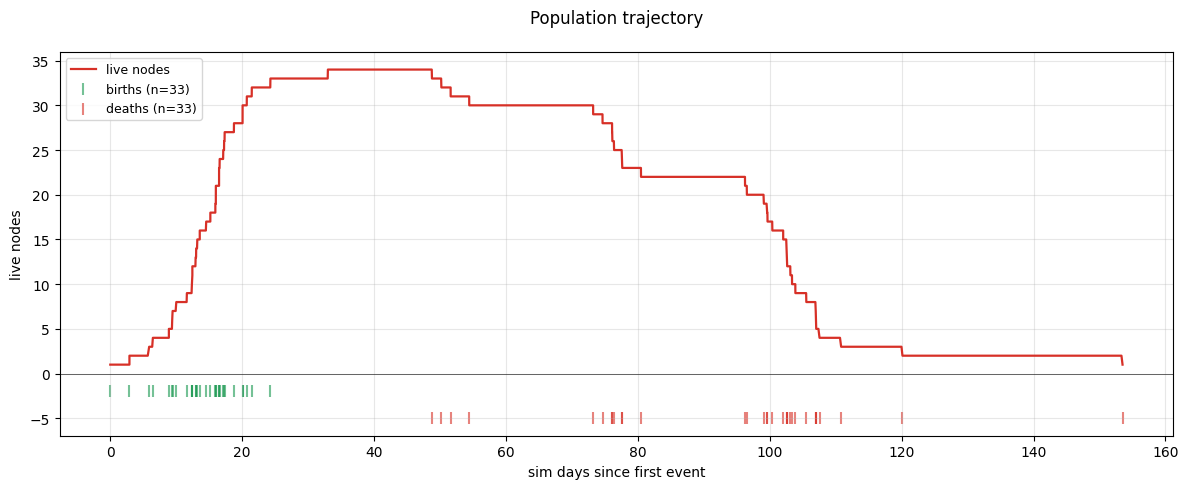
\includegraphics[width=0.6\linewidth]{figures/population_no_faucet.png}}
  \smallskip
  \small
  \begin{itemize}
    \item Every €3.27 buys exactly one day, so the fleet's
      \textbf{total lifespan is} at 3061 node-days (mean 93 days @ 33 nodes).
    \item One ``old'' survivor, as the failsafe concentrates residual funds into one node.
  \end{itemize}
  \textcolor{tud Orange}{\textbf{The closed-system prediction holds: a once-funded
  fleet cannot self-sustain.}}
\end{frame}
}


{
\setbeamerfont{itemize/enumerate body}{size=\small} % template pins lists to \normalsize
\begin{frame}{The lifespan clusters were predictable}
\smallskip
\smallskip
\smallskip
  \centerline{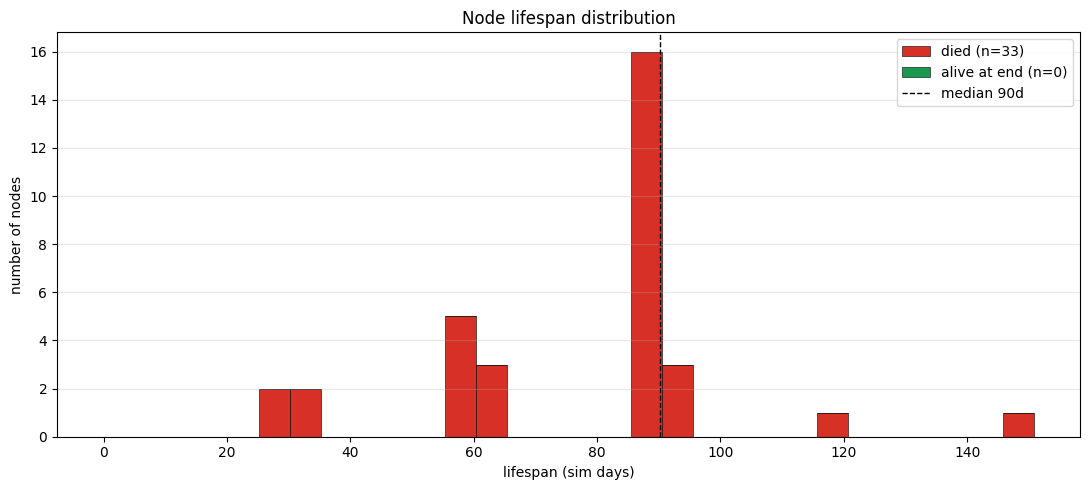
\includegraphics[width=0.65\linewidth]{figures/lifespan_hist_no_faucet.png}}

\small
Each cluster is a spawn constant: \textbf{90 d} is
      the post-spawn runway any parent retains. \textbf{60 d} and \textbf{30 d} are the last two generations of children.
  

  \begin{exampleblock}{Specification met}
    The cluster positions should be fixed, with the histogram confirming.
  \end{exampleblock}
\end{frame}
}


{
\setbeamerfont{itemize/enumerate body}{size=\small} % template pins lists to \normalsize
\begin{frame}{Income run: persistence, and an artifact}
  \framesubtitle{Open system}
  \centerline{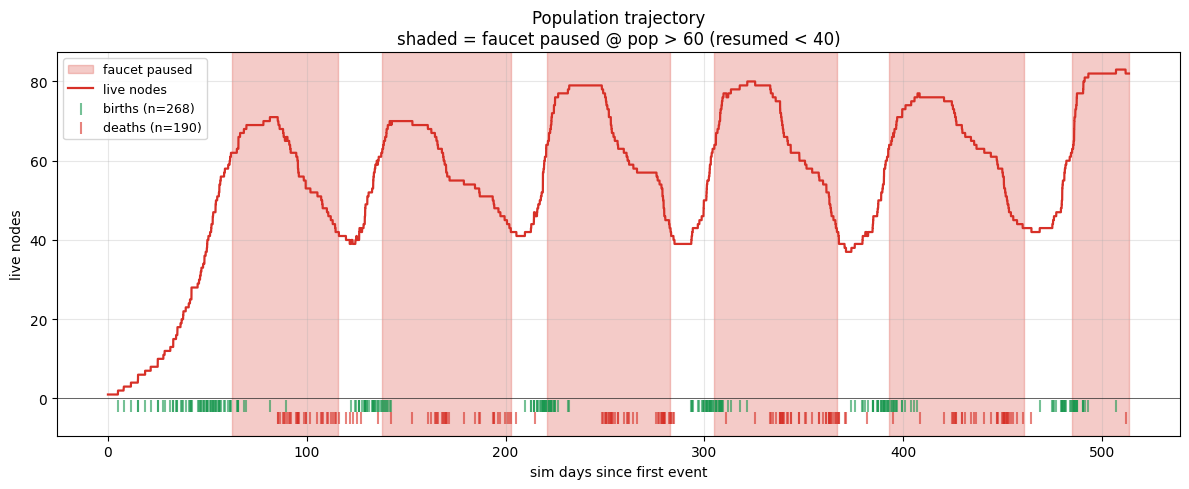
\includegraphics[width=0.54\linewidth]{figures/population_faucet.png}}
  \smallskip
  \small
  \begin{itemize}
    \item The 40--80 oscillation is an \textbf{artifact of the node cap}: the host
      tops out near 80 containers, so income is cut at 60 nodes and restored below
      40.
    \item Underneath hides a real self-limiting dynamic --- each spawn spreads
      capital over more nodes, shrinking per-node surplus --- but at these sizes the
      cap masks it (\(\to\) future work).
  \end{itemize}

  \textcolor{tud Orange}{\textbf{Income above per-node rent turns a 153-day die-off
  into persistence past 510 days.}}
\end{frame}
}


{
\setbeamerfont{itemize/enumerate body}{size=\small} % template pins lists to \normalsize
\begin{frame}{Survival without longevity}
  \framesubtitle{Lifespans, with income}
  \centerline{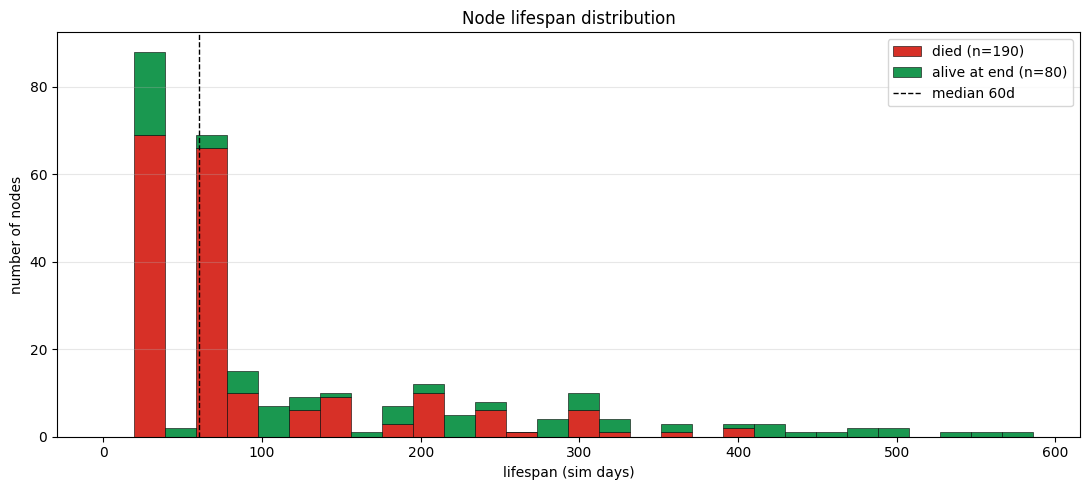
\includegraphics[width=0.42\linewidth]{figures/lifespan_hist_faucet.png}}
  \smallskip
  \small
  \begin{itemize}
    \item Uneven early income (Dirichlet shares) splits the fleet: a node drawing
      above-median income early crosses the spawn threshold with a large surplus and
      keeps 60\% of it, so \textbf{early wealth compounds} into a few long-lived
      lineages.
  \end{itemize}

  \begin{block}{The turnover principle}
    Survival needs only \emph{some} node holding a surplus, so a small well-funded
    minority replaces the short-lived majority --- the fleet tolerates high turnover
    by design.
  \end{block}
\end{frame}
}


{
\setbeamerfont{itemize/enumerate body}{size=\small} % template pins lists to \normalsize
\begin{frame}{Caution under selection: the hypothesis}
  \framesubtitle{Trait distribution of live nodes, 90-day snapshots}
  \small
  \begin{columns}[T, onlytextwidth]
    \begin{column}{0.46\textwidth}
      \centering
      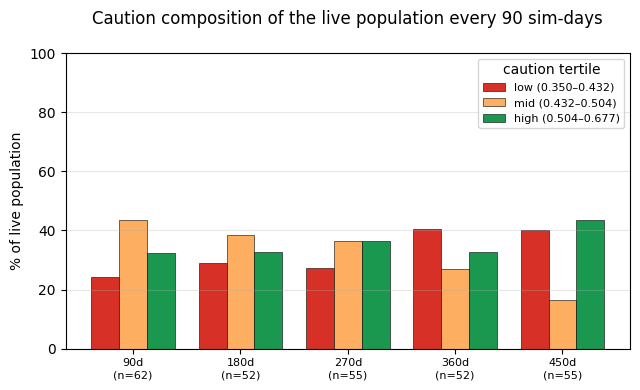
\includegraphics[width=\linewidth]{figures/caution_alive_tertiles_faucet.png}
    \end{column}
    \begin{column}{0.5\textwidth}
      Mutation is \textbf{mean-reverting toward 0.5}, yet the middle hollows while
      both extremes grow --- polarization against a centering pull means
      \textcolor{tud Orange}{genuine selection pressure} is acting.

      \smallskip
      \textbf{Hypothesis:} the income on/off cycle rewards opposite strategies ---
      low caution exploits growth (spawn aggressively), high caution survives
      drought (hoard runway), mid caution exploits neither.

      \smallskip
      Two falsifiable predictions:
      \begin{enumerate}
        \item low caution reproduces faster during income;
        \item high caution dies less during drought.
      \end{enumerate}
    \end{column}
  \end{columns}
\end{frame}
}


{
\setbeamerfont{itemize/enumerate body}{size=\small} % template pins lists to \normalsize
\begin{frame}{Caution under selection: the result}
  \framesubtitle{Birth and death rates by caution group and phase}
  \small
  \begin{columns}[T, onlytextwidth]
    \begin{column}{0.42\textwidth}
      \centering
      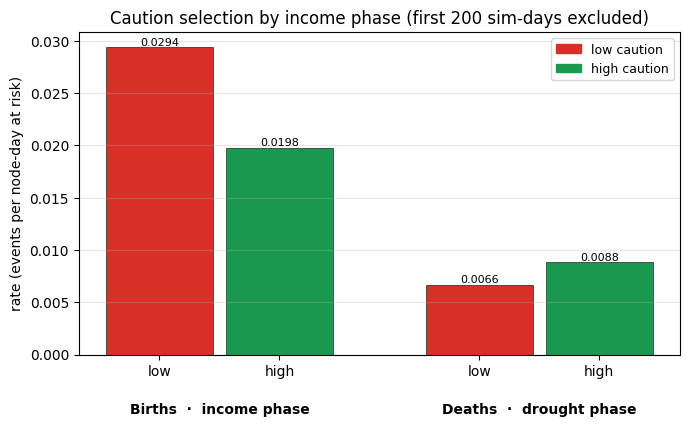
\includegraphics[width=\linewidth]{figures/caution_birth_death_diff.png}
    \end{column}
    \begin{column}{0.54\textwidth}
      \begin{exampleblock}{Prediction 1 --- confirmed}
        Low caution reproduces \(\sim\)50\% faster while income flows
        (0.0294 vs.\ 0.0198 births/day).
      \end{exampleblock}
      \begin{alertblock}{Prediction 2 --- disconfirmed}
        No survival edge --- high caution even dies slightly \emph{more} in drought
        (0.0088 vs.\ 0.0066 per day). Selection favored low caution: the reproduction
        gap ran in every phase.
      \end{alertblock}

      {\footnotesize The environment was \textbf{income-dominated} --- pauses too
      short for caution to pay off. The mechanism works; testing the survival half
      awaits sustained scarcity (\(\to\) future work).}
    \end{column}
  \end{columns}
\end{frame}
}
